\documentclass{article}

\usepackage{fullpage}
\usepackage{color}
\usepackage{amsmath}
\usepackage{url}
\usepackage{verbatim}
\usepackage{graphicx}
\usepackage{parskip}
\usepackage{amssymb}
\usepackage{nicefrac}
\usepackage{listings} % For displaying code
\usepackage{algorithm2e} % pseudo-code

% Answers
\def\ans#1{\par\gre{Answer: #1}}

% Colors
\definecolor{blu}{rgb}{0,0,1}
\def\blu#1{{\color{blu}#1}}
\definecolor{gre}{rgb}{0,.5,0}
\def\gre#1{{\color{gre}#1}}
\definecolor{red}{rgb}{1,0,0}
\def\red#1{{\color{red}#1}}
\def\norm#1{\|#1\|}

% Math
\def\R{\mathbb{R}}
\def\argmax{\mathop{\rm arg\,max}}
\def\argmin{\mathop{\rm arg\,min}}
\newcommand{\mat}[1]{\begin{bmatrix}#1\end{bmatrix}}
\newcommand{\alignStar}[1]{\begin{align*}#1\end{align*}}
\def\half{\frac 1 2}
\def\cond{\; | \;}

% LaTeX
\newcommand{\fig}[2]{\includegraphics[width=#1\textwidth]{a5f/#2}}
\newcommand{\centerfig}[2]{\begin{center}\includegraphics[width=#1\textwidth]{a5f/#2}\end{center}}
\def\items#1{\begin{itemize}#1\end{itemize}}
\def\enum#1{\begin{enumerate}#1\end{enumerate}}


\begin{document}

\title{CPSC 340 Assignment 5 (due Friday November 15 at 11:55pm)}
\author{}
\date{}
\maketitle
\vspace{-4em}


\red{If you are planning to do a poster project, make sure to register for the poster session as soon as possible. Details regarding registration are here:\\
\url{https://piazza.com/class/k02x04b6o524?cid=358}
}


\section{Kernel Trick}

In this question you will revisit questions from previous assignments, this time implementing the same (or similar) models using the ``kernel trick''.

\subsection{``Other'' Normal Equations}

The script \emph{example\_nonLinear} loads a dataset from a previous assignment, and fits an L2-regularized least squares model with a bias term (the regularization leads to small improvement in the test error, even for this 2-variable problem). Modify the \emph{leastSquaresBiasL2} function so that it uses the ``other'' normal equations we discussed in class,
\[
v = Z^T\underbrace{(ZZ^T + \lambda I)^{-1}y}_u.
\]
In particular, the training should result in an $n \times 1$ vetor $u$ of parameters, and predictions are made based on the training $Z$ and the vector $u$. \blu{Hand in your code for the modified function}.

Hint: you should get the same predictions as the original funciton. To help debugging, you may want to first re-write the calculation of $v$ using the above formula, to verify that this gives you the same vector $v$.
\ans{
\includegraphics[width=10cm]{Q11.png}}

\subsection{Polynomial Kernel}

Write a new function, \emph{leastSquaresKernelBasis}, taking a degree $p$ and a regularization parameter $\lambda$. It should fit a degree-$p$ polynomial to the data, using the kernel trick to avoid ever forming the matrix $Z$. \blu{Hand in your code and the plot obtained with $p=3$ and $\lambda =10^{-6}$.}

Hint: you may find it helpful to write a function \emph{polyKernel} that takes two matrices as inputs (either $X$ and $X$ or $\tilde{X}$ and $X$) and a degree $p$, and computes the polynomial kernel between all pairs of rows in the matrices.
\ans{\\
    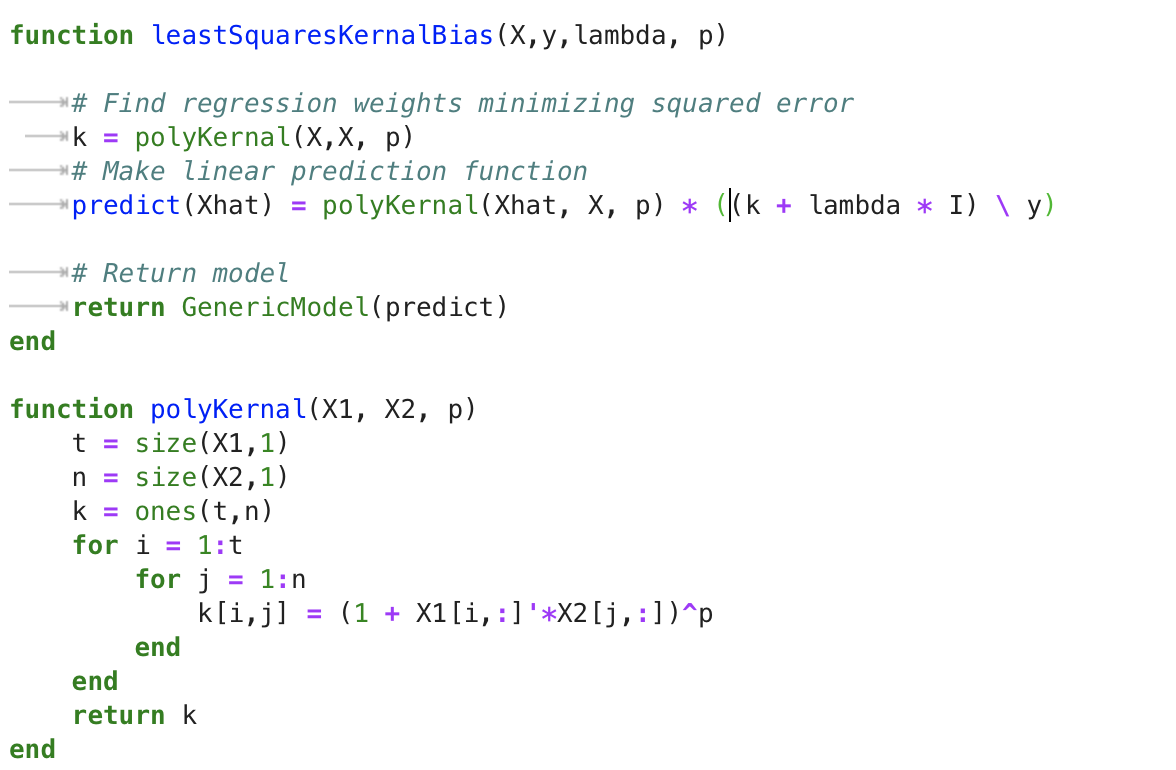
\includegraphics[width=10cm]{Q12.png}\\
    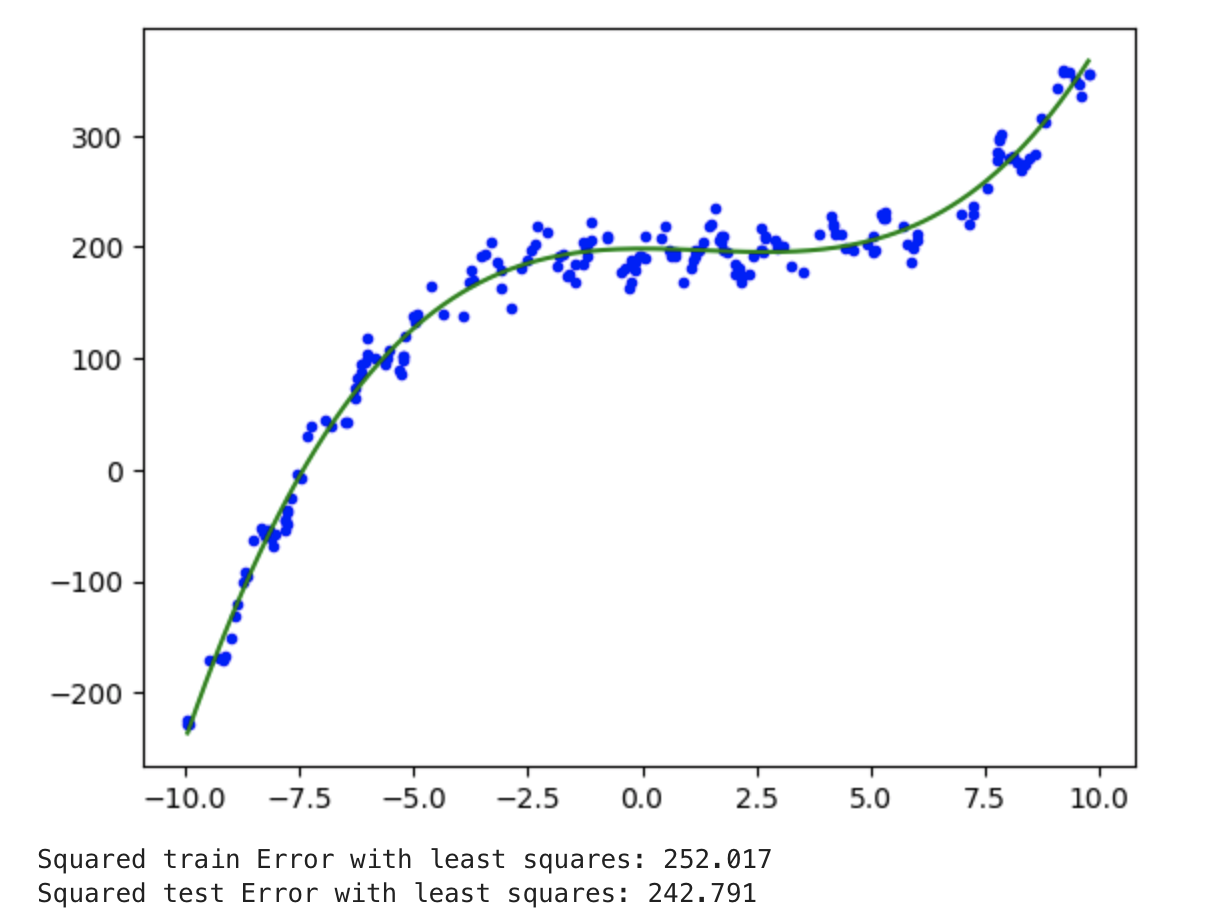
\includegraphics[width=10cm]{Q13.png}
}

\subsection{Gaussian-RBF Kernel}

\blu{Repeat the previous question and report the same quantities, but using the Gaussian RBF kernel.} You can use $\sigma=1$ and $\lambda=10^{-6}$ for the plot.
\ans{
    \\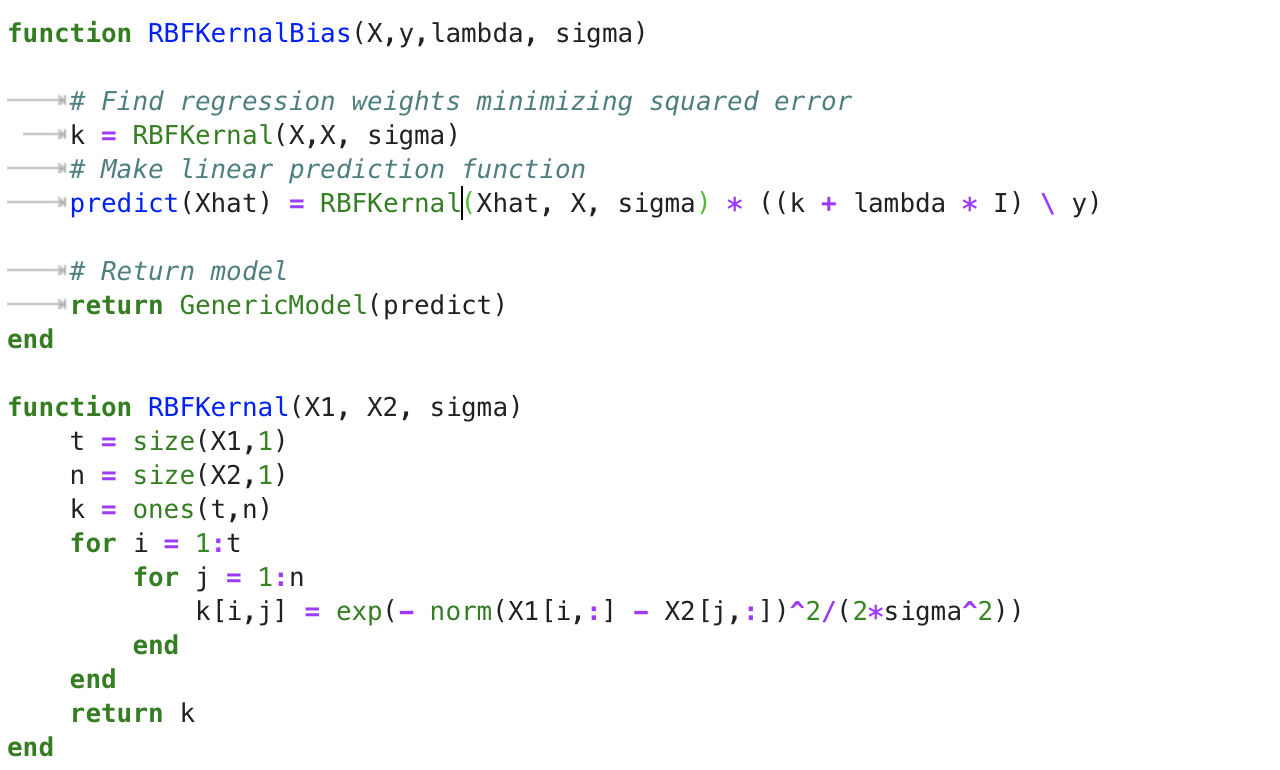
\includegraphics[width=10cm]{Q14.png}\\
    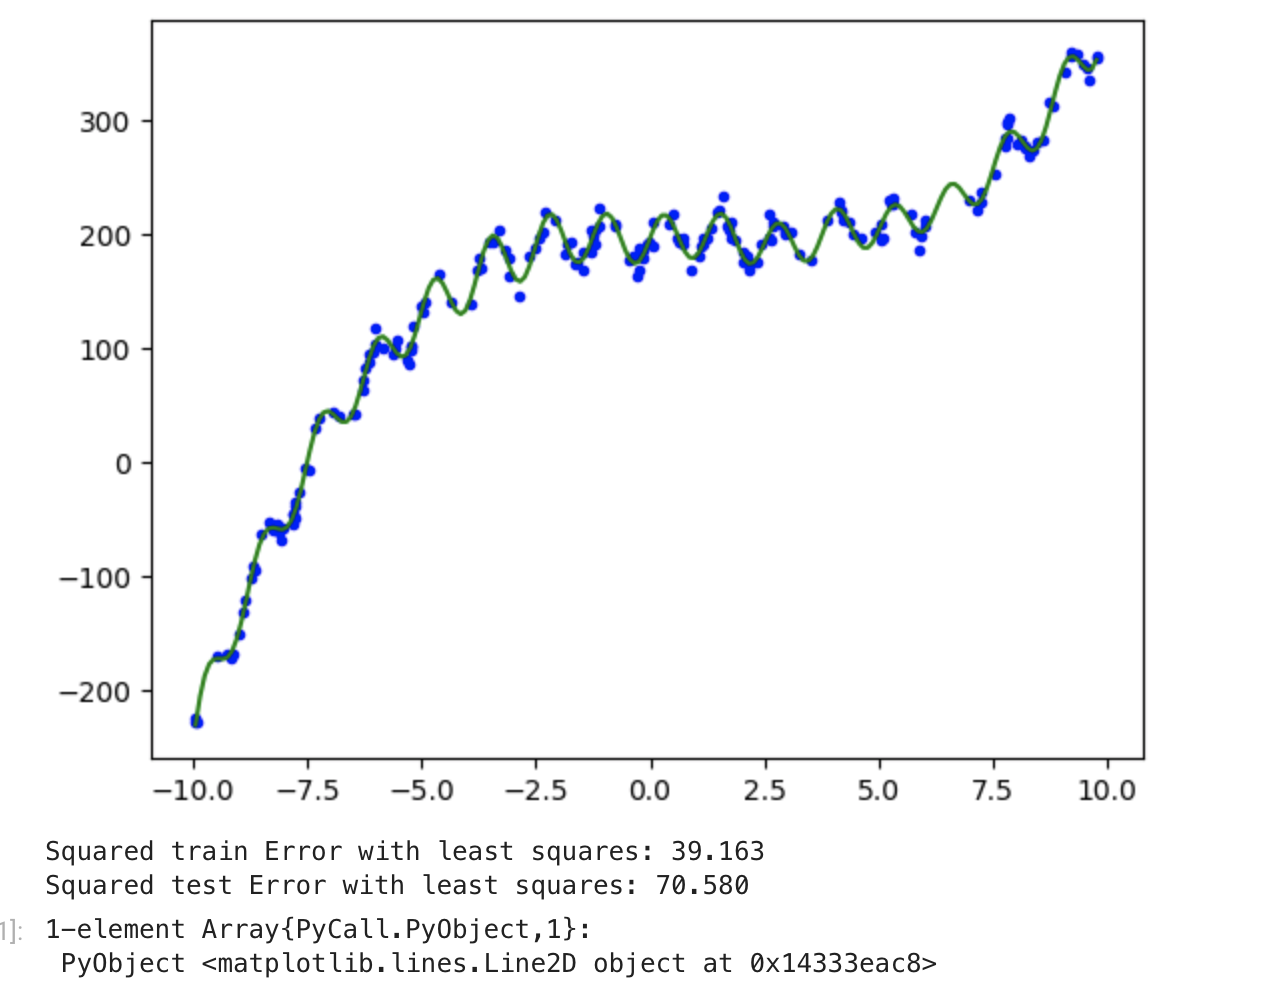
\includegraphics[width=10cm]{Q15.png}
    }


\section{MAP Estimation}

In class, we considered MAP estimation in a regression model where we assumed that:
\items{
\item The likelihood $p(y_i \cond x_i, w)$ for each example $i$ is a normal distribution with a mean of $w^Tx_i$ and a variance of $1$.
\item The prior $p(w_j)$ for each variable $j$ is a normal distribution with a mean of zero and a variance of $\lambda^{-1}$.
}
Under these assumptions we showed that computing the MAP estimate with $n$ training examples leads to the standard L2-regularized least squares objective function:
\[
f(w) = \frac{1}{2}\norm{Xw - y}^2 + \frac \lambda 2 \norm{w}^2.
\]
\blu{For each of the alternate assumptions below, write down the objective function that results} (from minimizing the negative log-posterior, and simplifying as much as possible):
\enum{
\item  We use a Laplace likelihood with a mean of $w^Tx_i$ and a scale of $1$, and we use a zero-mean Laplace prior for each variable with a scale parameter of $\lambda^{-1}$,
\[
p(y_i \cond x_i, w) = \frac 1 2 \exp(-|w^Tx_i - y_i|), \quad  p(w_j) = \frac{\lambda}{2}\exp(-\lambda|w_j|).
\]
\ans{
    \begin{align*}
    f(w) &= -\sum_{i=1}^n \log(p(y_i \cond x_i, w))\\
    &=- \sum_{i=1}^n \log(\frac 1 2 \exp(-|w^Tx_i - y_i|))\\
    &= - \sum_{i=1}^n \log(\frac 1 2) - \sum_{i=1}^n \log(\exp(-|w^Tx_i - y_i|)) \\
    &= contant - \sum_{i=1}^n -|w^Tx_i - y_i|\\
    & = constant + \|w^Tx - y\|_1
\end{align*}
}
\item We use a normal  likelihood with a mean of $w^Tx_i$ but where each example $i$ has its own  positive variance $\sigma_i^2$, and a normal prior with a variance of $\lambda^{-1}$ and a mean that is some ``guess'' $w^0$ of the optimal parameter vector,
\[
p(y_i \cond x_i,w) = \frac{1}{\sqrt{2\sigma_i^2\pi}}\exp\left(-\frac{(w^Tx_i - y_i)^2}{2\sigma_i^2}\right), \quad p(w_j) \propto \exp\left(-\frac{\lambda(w_j -  w^0_j)^2}{2}\right).
\]
\ans{
    \begin{align*}
        f(w) &= -\sum_{i=1}^n \log(p(y_i \cond x_i, w))\\
        & = -\sum_{i=1}^n \log(\frac{1}{\sqrt{2\sigma_i^2\pi}}\exp\left(-\frac{(w^Tx_i - y_i)^2}{2\sigma_i^2}\right)) \\
        & = -\sum_{i=1}^n (\log(\frac{1}{\sqrt{2\sigma_i^2\pi}}) + \log(\exp\left(-\frac{(w^Tx_i - y_i)^2}{2\sigma_i^2}\right)))\\
        & = -\sum_{i=1}^n (constant + \left(-\frac{(w^Tx_i - y_i)^2}{2\sigma_i^2}\right))) \\
        & = constant + \|{\Sigma^{-1}(w^Tx - y)}\|_2^2
    \end{align*}
}
The standard notation for this case is to use $\Sigma$ as a diagonal matrix with the $\sigma_i^2$ values along the diagonal.
\item We use a Poisson likelihood with a mean of $\exp(w^Tx_i)$,\footnote{This is one way to use regression to model \emph{counts}, like ``number of Facebook likes''.} and we use a uniform prior for some constant $\kappa$,
\[
p(y_i \cond x_i, w) = \frac{\exp(y_iw^Tx_i)\exp(-\exp(w^Tx_i))}{y_i!}, \quad p(w_j) \propto \kappa
\]
\ans{
\begin{align*}
    f(w) &= -\sum_{i=1}^n \log(p(y_i \cond x_i, w))\\
    & = -\sum_{i=1}^n \log(\frac{\exp(y_iw^Tx_i)\exp(-\exp(w^Tx_i))}{y_i!})\\
    & = -\sum_{i=1}^n y_iw^Tx_i + -\exp(w^Tx_i) - \log(y_i!)
\end{align*}
}
For this sub-question you don't need to put likelihood in matrix notation.
\item We use a Laplace likelihood with a mean of $w^Tx_i$ where each example $i$ has its own positive scale paramater $v_i^{-1}$, and a  student $t$ prior (which is very robust to irrelevant features) with $\nu$ degrees of freedom,
\[
p(y_i \cond x_i, w) = \frac 1 2 \exp\left(-v_i|w^Tx_i - y_i|\right), \quad  p(w_j) = \frac{\Gamma\left(\frac{\nu + 1}{2}\right)}{\sqrt{\nu\pi}\Gamma\left(\frac \nu 2\right)}\left(1 + \frac{w_j^2}{\nu}\right)^{-\frac{\nu+1}{2}}
\]
where you use can $V$ as a diagonal matrix with the $v_i$ along the diagonal and $\Gamma$ is the ``gamma" function (which is always non-negative). You do not need to put the log-prior in matrix notation.
\ans{
    \begin{align*}
        f(w) &= -\sum_{i=1}^n \log(p(y_i \cond x_i, w))\\
        & = -\sum_{i=1}^n \log(\frac 1 2 \exp\left(-v_i|w^Tx_i - y_i|\right))\\
        & = -\sum_{i=1}^n \log(1/2) + \log(\exp\left(-v_i|w^Tx_i - y_i|\right)) \\
        & = constant -\sum_{i=1}^n \left(-v_i|w^Tx_i - y_i|\right)\\
        &= constant + \|(w^TX -y)V\|_1
    \end{align*}
}
}



\section{Principal Component Analysis}

\subsection{PCA by Hand}

Consider the following dataset, containing 5 examples with 2 features each:
\begin{center}
\begin{tabular}{cc}
$x_1$ & $x_2$\\
\hline
-4 & 3\\
0 & 1\\
-2 & 2\\
4 & -1\\
2 & 0\\
\end{tabular}
\end{center}
Recall that with PCA we usually assume that the PCs are normalized ($\norm{w} = 1$), that we need to center the data before we apply PCA, and that the direction of the first PC is the one that minimizes the orthogonal distance to all data points.
\blu{
\enum{
\item What is the first principal component?
\ans{
    Normalize X: ($X_2-1$) \\
    \begin{tabular}{cc}
        $x_1$ & $x_2$\\
        \hline
        -4 & 2\\
        0 & 0\\
        -2 & 1\\
        4 & -2\\
        2 & -1\\
        \end{tabular}
    Then we can see the line is $x_2 = -\frac {x_1} 2$. \\
    We then can have $W = [-2, 1]^T$
}
\item What is the (L2-norm) reconstruction error of the point (-3, 2.5)? (Show your work.)
\ans{We first do the "normalize". We get data: (-3,1.5) \\
Thus We can see that reconstruction is $ 1.5 * [-2, 1]^T + [0, 1]$
}
\item What is the (L2-norm) reconstruction error of the point (-3, 2)? (Show your work.)
\ans{
    We first do the "normalize". We get data: (-3,1) 
The slope of line that is certical to $x_2 = -\frac{x_1} 2$ is $2 x_1 = x_2$. We plug (-3,1) in to the equation \\
$2x_1 = x_2 + c$ we can resolve that c = -8. We then would get the intersection of the current line to w.\\
    We have \[\begin{cases}
        x_2 = -\frac{x_1} 2 \\
        2x_1 = x_2 - 7
    \end{cases}\]
\[\begin{cases} 
    x1 = - \frac {14} 5 \\
    x2 = \frac{7} {5}
\end{cases}\]
Thus the reconstruction is $ \frac{7} {5} * [-2, 1]^T + [0, 1]= [-2.8, 2.4]$
}
}
}




\subsection{Data Visualization}

The script \emph{example\_PCA} will load a dataset containing 50 examples, each representing an animal. The 85 features are traits of these animals. The script standardizes these features and gives two unsatisfying visualizations of it. First it shows a plot of the matrix entries, which has too much information and thus gives little insight into the relationships between the animals. Next it shows a scatterplot based on two random features and displays the name of 10 randomly-chosen animals. Because of the binary features even a scatterplot matrix shows us almost nothing about the data.

The function \emph{PCA} applies the classic PCA method (orthogonal bases via SVD) for a given $k$. Using this function, modify the demo so that the scatterplot uses the latent features $z_i$ from the PCA model with $k=2$. Make a scatterplot of the two columns in $Z$, and use the \emph{annotate} function to label a bunch of the points in the scatterplot.
\blu{
\enum{
\item  Hand in your modified demo and the scatterplot.
\ans{\\
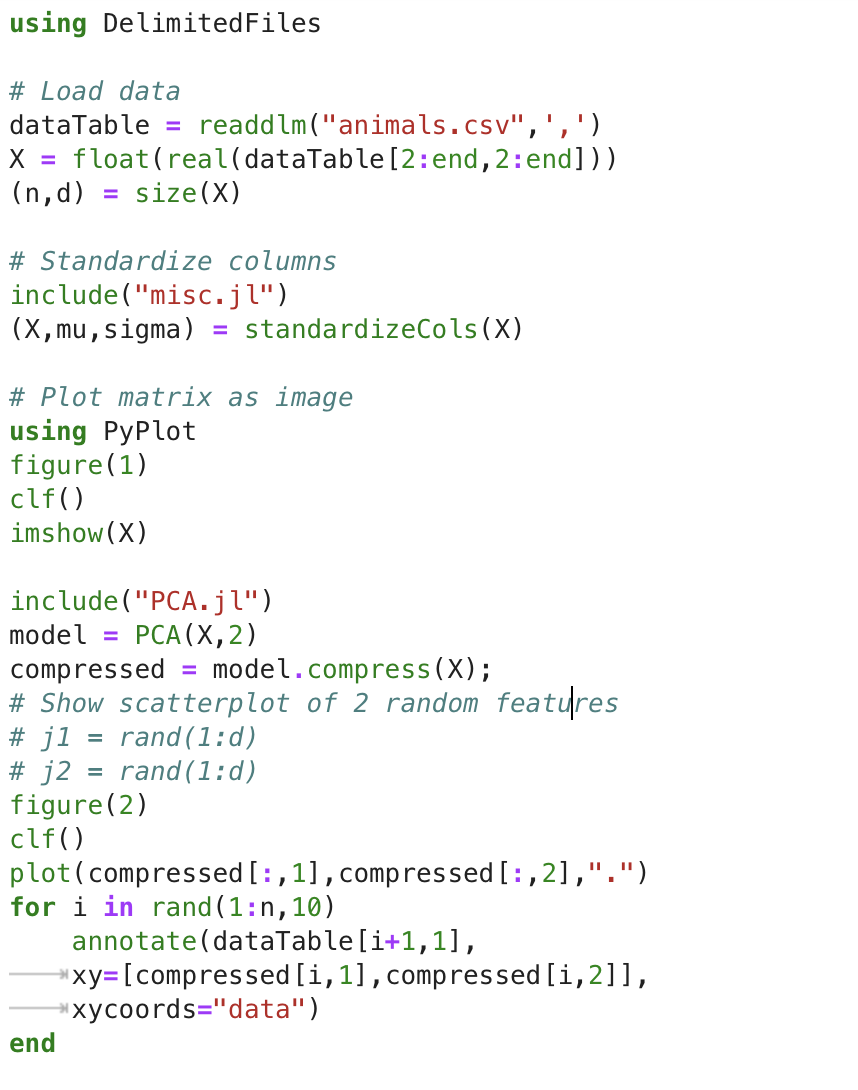
\includegraphics[width=10cm]{Q32Code.png}\\
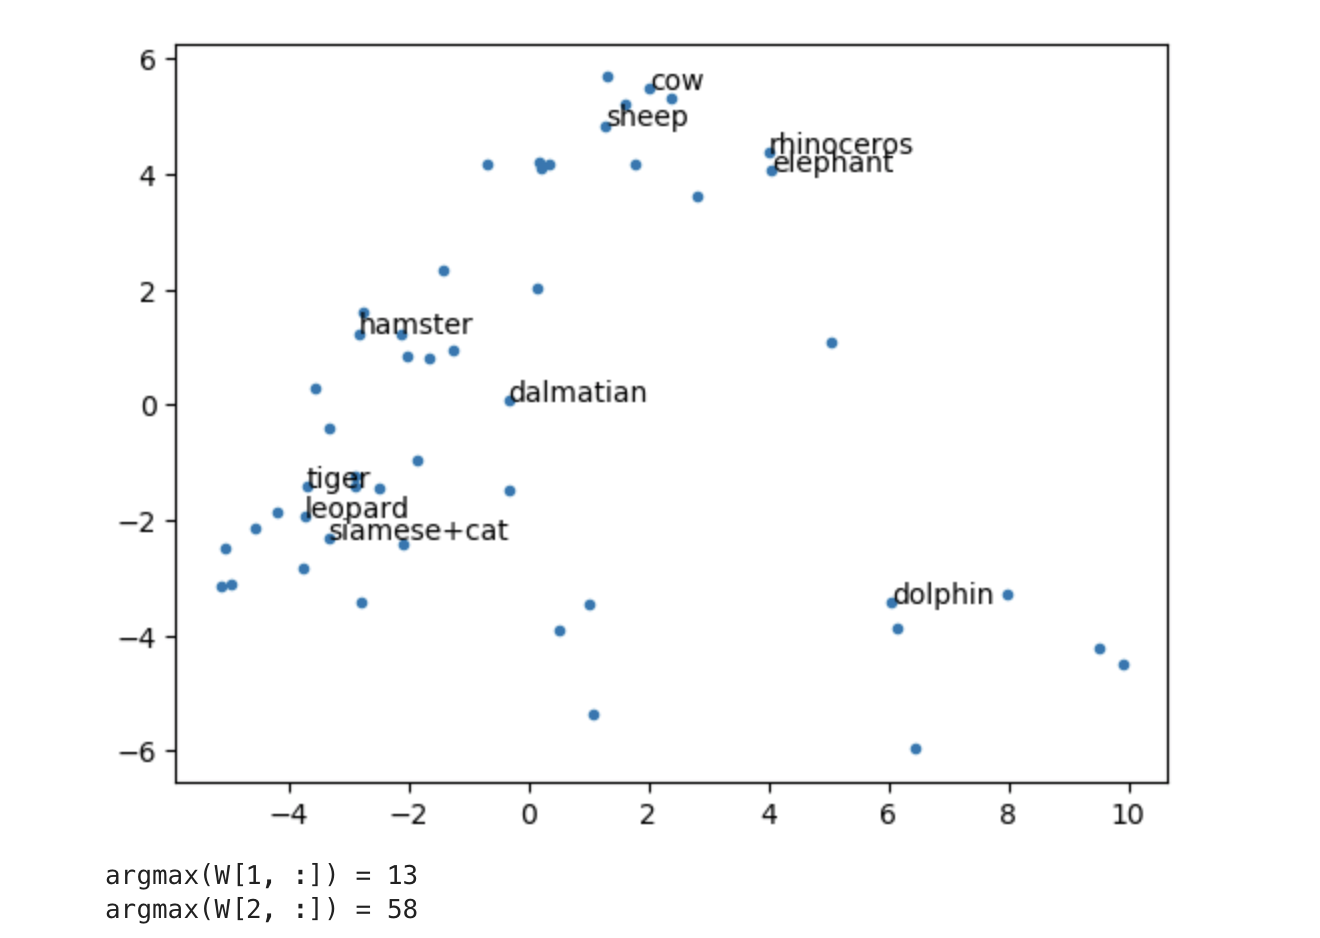
\includegraphics[width=10cm]{Q321.png}}
\item Which trait of the animals has the largest influence (absolute value) on the first principal component? (Make sure not to forget the ``+1'' when looking for the name of the trait in the \emph{dataTable}).
\ans{
    "hairless"
}
\item Which trait of the animals has the largest influence (absolute value) on the second principal component?
\ans{
    "grazer"
}}
}


\subsection{Data Compression}

It is important to know how much of the information in our dataset is captured by the low-dimensional PCA representation.
In class we discussed the ``analysis" view that PCA maximizes the variance that is explained by the PCs, and the connection between the Frobenius norm and the variance of a centered data matrix $X$. Use this connection to answer the following:
\blu{\enum{
\item How much of the variance is explained by our two-dimensional representation from the previous question?
\ans{$1 - \frac {\|ZW - X\|^2} {\|x\|^2} = 1 - 0.8355 = 0.1645$} 
\item How many\ PCs are required to explain 50\% of the variance in the data?
\ans{14}
}}
Note: you can compute the Frobenius norm of a matrix using the function \emph{norm}. Also, note that the ``variance explained'' formula from class assumes that $X$ is already centered.



\section{Very-Short Answer Questions}


\enum{
\item What is the difference between multi-label and multi-class classification?
\item We discussed ``global'' vs. ``local'' features for e-mail classification. What is an advantage of using global features, and what is advantage of using local features?
\ans{"Global Features are useful when we have an important email for all users. And Local features are useful for identifying emails for specific users.}
\item Assuming we want to use the original features (no change of basis) in a linear model, what is an advantage of the ``other'' normal equations over the original normal equations?
\ans{It is faster when $n<d$.}
\item What is the key advantage of stochastic gradient methods over gradient descent methods?
\ans{Solve the issue when "n" is really large and it will take a long time for gradiant decent to take one step.}
\item Which of the following step-size sequences lead to convergence of stochastic gradient to a stationary point?
\enum{
\item $\alpha^t = 1/t^2$.
\item $\alpha^t = 1/t$.
\item $\alpha^t = \gamma/t$ (for $\gamma > 0$).
\item $\alpha^t = 1/(t+\gamma)$ (for $\gamma > 0$).
\item $\alpha^t = 1/\sqrt{t}$.
\item $\alpha^t = 1$.
}
\ans{b,c,d}
\item In the language of loss functions and regularization, what is the difference between MLE and MAP?
\ans{MAP will give a score of the likelihood of w as perior, which is like the regularization, what gives a very samll value for the w that is likely to be overfitting. }
\item What is the difference between a generative model and a discriminative model?
\item In the MLE framework, what is the connection between the logistic loss and the sigmoid function in linear models.
\ans{If we use sigmoid function, we will get logistic loss after applying the MLE.}
\item What is the significance of choosing $k=2$ for visualizing with PCA.
\ans{We can plot it using the 2 "features" to get a better visualization, than 2 original features.}
\item With PCA, is it possible for the loss to increase if $k$ is increased? Briefly justify your answer.
\ans{No. Because you can always set Z value to 0 to the k that is more than the previous one and get the same loss.}
\item Why doesn't it make sense to do PCA with $k > d$?
\ans{Because you will always get a perfect result.}
\item In terms of the matrices associated with PCA ($X$, $W$, $Z$, $\hat{X}$), where would an ``eigenface'' be stored?
\ans{W}
}


\section*{Project Update (OPTIONAL for 340 STUDENTS)}

Alongside Assignment 5, we are also asking you to submit a \emph{project update}. It's ok if you haven't yet made much progress on your project, but we're making you submit this document as an excuse to get together with your project and plan. In particular, the project update should be a 1-page report covering the following:
\enum{
\item \textbf{What has been done already}: for example, you might have already found a group of appropriate size, picked a topic, got access to appropriate data, read some related papers, or maybe even ran some preliminary experiments.
\item \textbf{What still needs to be}: what are the ``action items'' that need to be finished in order to complete the project. The purpose here is that you make a plan to finishing the different things that will need to come together in order to finish your project.
}
It's ok if the report is fairly short, and just written as series of bullet items addressing the two issues above.



\end{document}